\documentclass[10pt,landscape]{article}
\usepackage[letterpaper,landscape,margin=0.42in]{geometry}
\usepackage[T1]{fontenc}
\usepackage{lmodern}
\usepackage{amsmath,amssymb,mathtools}
\usepackage{xcolor}
\usepackage{tikz}
\usepackage{graphicx}
\usetikzlibrary{arrows.meta,positioning,calc,fit,backgrounds,shapes.geometric,decorations.pathreplacing}
\pagestyle{empty}
\setlength{\parindent}{0pt}
\setlength{\parskip}{0pt}

\definecolor{ink}{HTML}{172033}
\definecolor{muted}{HTML}{64748B}
\definecolor{linegray}{HTML}{CBD5E1}
\definecolor{paper}{HTML}{F8FAFC}
\definecolor{blue}{HTML}{2563EB}
\definecolor{bluepale}{HTML}{EAF2FF}
\definecolor{teal}{HTML}{0F8B8D}
\definecolor{tealpale}{HTML}{E6F7F5}
\definecolor{amber}{HTML}{D97706}
\definecolor{amberpale}{HTML}{FFF4D6}
\definecolor{violet}{HTML}{7C3AED}
\definecolor{violetpale}{HTML}{F2EAFF}
\definecolor{green}{HTML}{16825D}
\definecolor{greenpale}{HTML}{E7F7EF}
\definecolor{rose}{HTML}{D43F66}
\definecolor{rosepale}{HTML}{FFEAF0}

\tikzset{
  >={Stealth[length=2.3mm,width=1.55mm]},
  card/.style={draw=linegray,rounded corners=2.5mm,fill=white,line width=.65pt},
  pill/.style={rounded corners=1.8mm,inner xsep=2.8mm,inner ysep=1.2mm,font=\bfseries\small},
  flow/.style={->,line width=1.05pt,color=muted},
  strongflow/.style={->,line width=1.7pt,color=blue},
  point/.style={circle,minimum size=3.5mm,inner sep=0pt,draw=ink,fill=white,line width=.7pt},
  diagpoint/.style={circle,minimum size=4.1mm,inner sep=0pt,draw=green,fill=greenpale,line width=1.1pt},
  code/.style={font=\ttfamily\small,anchor=west},
}

\newcommand{\Title}[2]{%
  {\fontsize{22}{24}\selectfont\bfseries\color{ink}#1}\hfill
  \tikz[baseline=-.65ex]\node[pill,fill=#2!12,text=#2]{PR 1 \enspace COMPLETE LATTICES};
  \par\vspace{1mm}\color{linegray}\rule{\linewidth}{0.8pt}\color{ink}\vspace{2mm}}
\newcommand{\Su}{\mathop{\textstyle\bigvee}}
\newcommand{\In}{\mathop{\textstyle\bigwedge}}
\newcommand{\lean}[1]{\texttt{#1}}
\newcommand{\isupdiag}{\texttt{iSup}\raisebox{-.22ex}{\scriptsize\texttt{2}}\texttt{\_eq\_iSup\_diagonal}}
\newcommand{\iinfdiag}{\texttt{iInf}\raisebox{-.22ex}{\scriptsize\texttt{2}}\texttt{\_eq\_iInf\_diagonal}}
\newcommand{\bigidea}[1]{%
  \begin{tikzpicture}
    \node[pill,fill=ink,text=white] (b) {BIG IDEA};
    \node[anchor=west,font=\bfseries\large,text=ink] at ($(b.east)+(0.35,0)$) {#1};
  \end{tikzpicture}}

\begin{document}
\color{ink}

% ------------------------------------------------------------------
% PAGE 1
\Title{A whole grid can collapse to its diagonal}{blue}

\begin{minipage}[t]{0.60\linewidth}
\resizebox{\linewidth}{!}{%
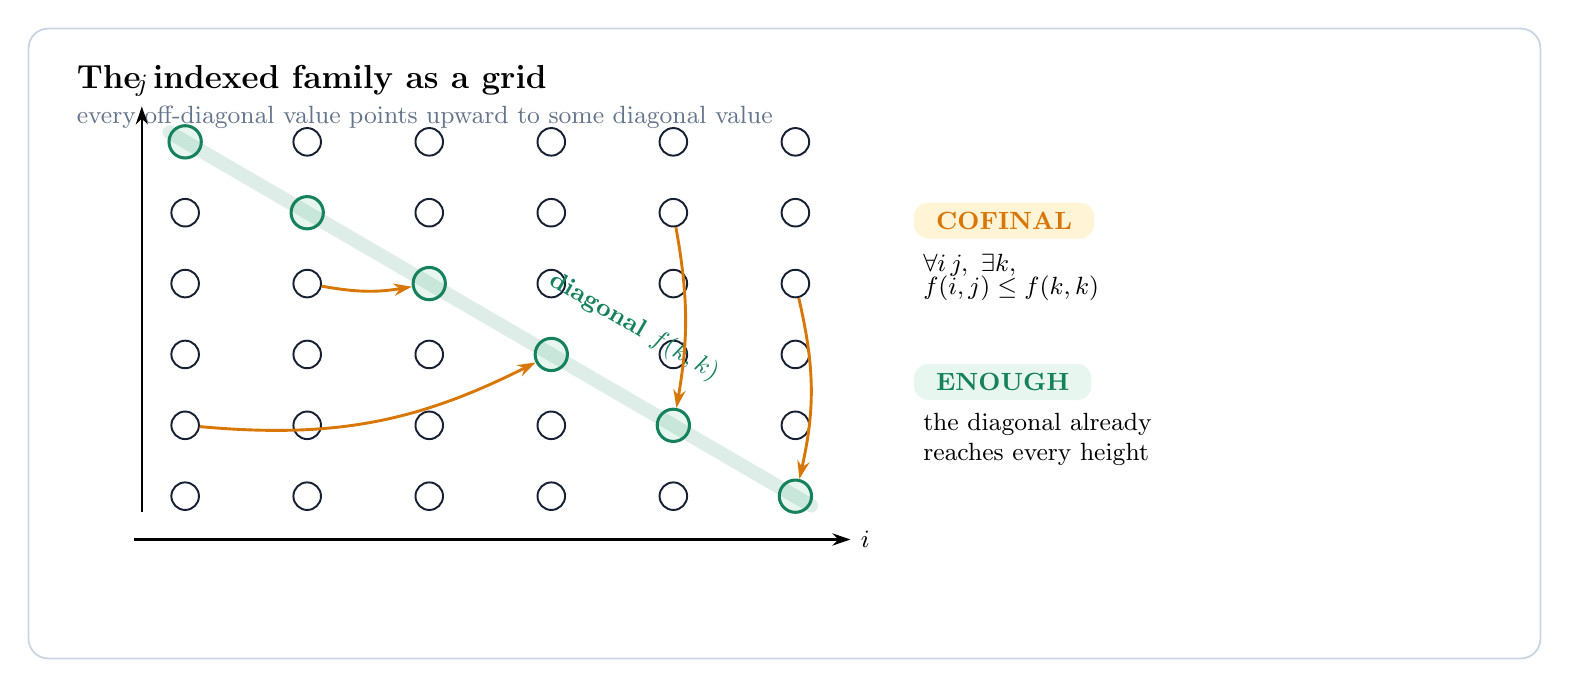
\begin{tikzpicture}[x=1cm,y=1cm]
  \node[card,minimum width=19.2cm,minimum height=8.0cm,anchor=north west] at (0,0) {};
  \node[anchor=north west,font=\bfseries\large] at (.5,-.35) {The indexed family as a grid};
  \node[anchor=north west,font=\small,text=muted] at (.5,-.87)
    {every off-diagonal value points upward to some diagonal value};

  \begin{scope}[shift={(2.0,-1.45)}]
    \foreach \i in {0,...,5}{
      \foreach \j in {0,...,5}{
        \ifnum\i=\j
          \node[diagpoint] (p\i\j) at (1.55*\i,-.9*\j) {};
        \else
          \node[point] (p\i\j) at (1.55*\i,-.9*\j) {};
        \fi
      }
    }
    \draw[->,line width=.85pt] (-.65,-5.05)--(8.45,-5.05) node[right,font=\small] {$i$};
    \draw[->,line width=.85pt] (-.55,-4.7)--(-.55,.45) node[above,font=\small] {$j$};
    \draw[green,line width=5pt,opacity=.14,line cap=round] (-.2,.12)--(7.95,-4.62);
    \node[rotate=-30,text=green,font=\bfseries\small] at (5.7,-2.35) {diagonal $f(k,k)$};
    \draw[flow,amber] (p04) to[bend right=16] (p33);
    \draw[flow,amber] (p12) to[bend right=10] (p22);
    \draw[flow,amber] (p41) to[bend left=10] (p44);
    \draw[flow,amber] (p52) to[bend left=13] (p55);
    \node[pill,fill=amberpale,text=amber,anchor=west] at (9.25,-1.0) {COFINAL};
    \node[anchor=west,align=left,font=\small] at (9.25,-1.72)
      {$\forall i\,j,\ \exists k,$\\[-1mm]$f(i,j)\le f(k,k)$};
    \node[pill,fill=greenpale,text=green,anchor=west] at (9.25,-3.05) {ENOUGH};
    \node[anchor=west,align=left,font=\small] at (9.25,-3.78)
      {the diagonal already\\reaches every height};
  \end{scope}
\end{tikzpicture}}
\end{minipage}\hfill
\begin{minipage}[t]{0.385\linewidth}
\resizebox{\linewidth}{!}{%
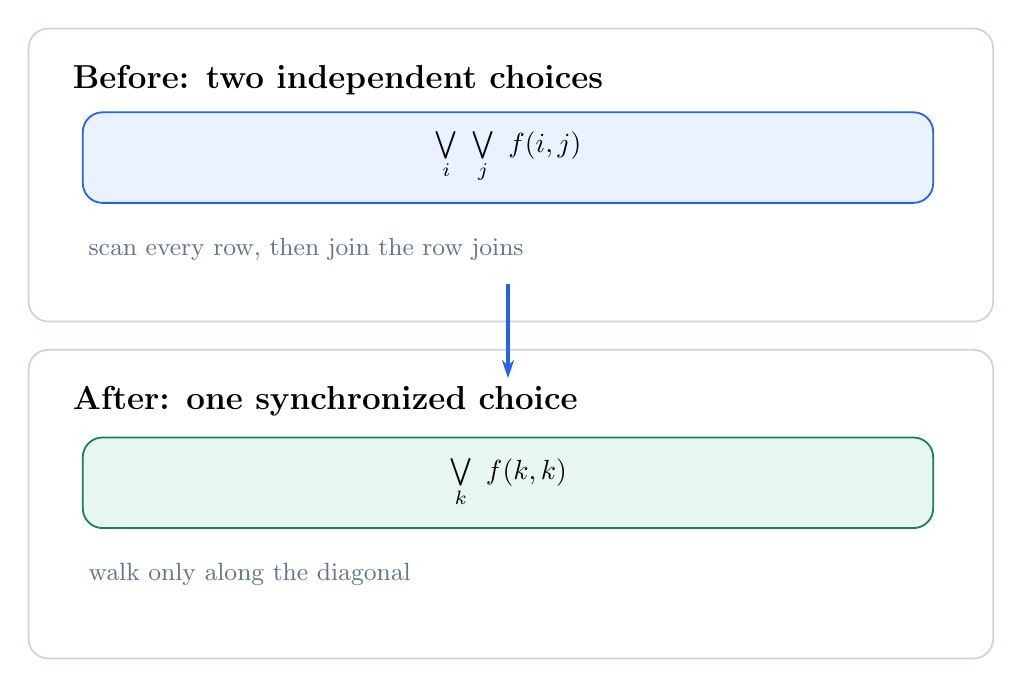
\begin{tikzpicture}[x=1cm,y=1cm]
  \node[card,minimum width=12.25cm,minimum height=3.72cm,anchor=north west] at (0,0) {};
  \node[anchor=north west,font=\bfseries\large] at (.45,-.35) {Before: two independent choices};
  \node[card,fill=bluepale,draw=blue,minimum width=10.8cm,minimum height=1.15cm] at (6.1,-1.65)
    {$\displaystyle \Su_i\ \Su_j\ f(i,j)$};
  \node[anchor=north west,font=\small,text=muted,align=left] at (.65,-2.55)
    {scan every row, then join the row joins};

  \node[card,minimum width=12.25cm,minimum height=3.92cm,anchor=north west] at (0,-4.08) {};
  \node[anchor=north west,font=\bfseries\large] at (.45,-4.43) {After: one synchronized choice};
  \node[card,fill=greenpale,draw=green,minimum width=10.8cm,minimum height=1.15cm] at (6.1,-5.78)
    {$\displaystyle \Su_k\ f(k,k)$};
  \node[anchor=north west,font=\small,text=muted,align=left] at (.65,-6.68)
    {walk only along the diagonal};
  \draw[strongflow] (6.1,-3.25)--(6.1,-4.45);
\end{tikzpicture}}
\end{minipage}

\vfill
\begin{center}

\begin{tikzpicture}
  \node[card,fill=greenpale,draw=green,minimum width=.91\linewidth,minimum height=1.05cm]
    {\Large\bfseries $\left(\displaystyle\bigvee_i\ \bigvee_j f(i,j)\right)
      =\displaystyle\bigvee_k f(k,k)$};
  \node[pill,fill=green,text=white,anchor=east] at (.475\linewidth,0) {\isupdiag};
\end{tikzpicture}
\end{center}

\newpage

% ------------------------------------------------------------------
% PAGE 2
\Title{Why the equality is true: two inequalities}{teal}

\begin{minipage}[t]{0.49\linewidth}
\resizebox{\linewidth}{!}{%
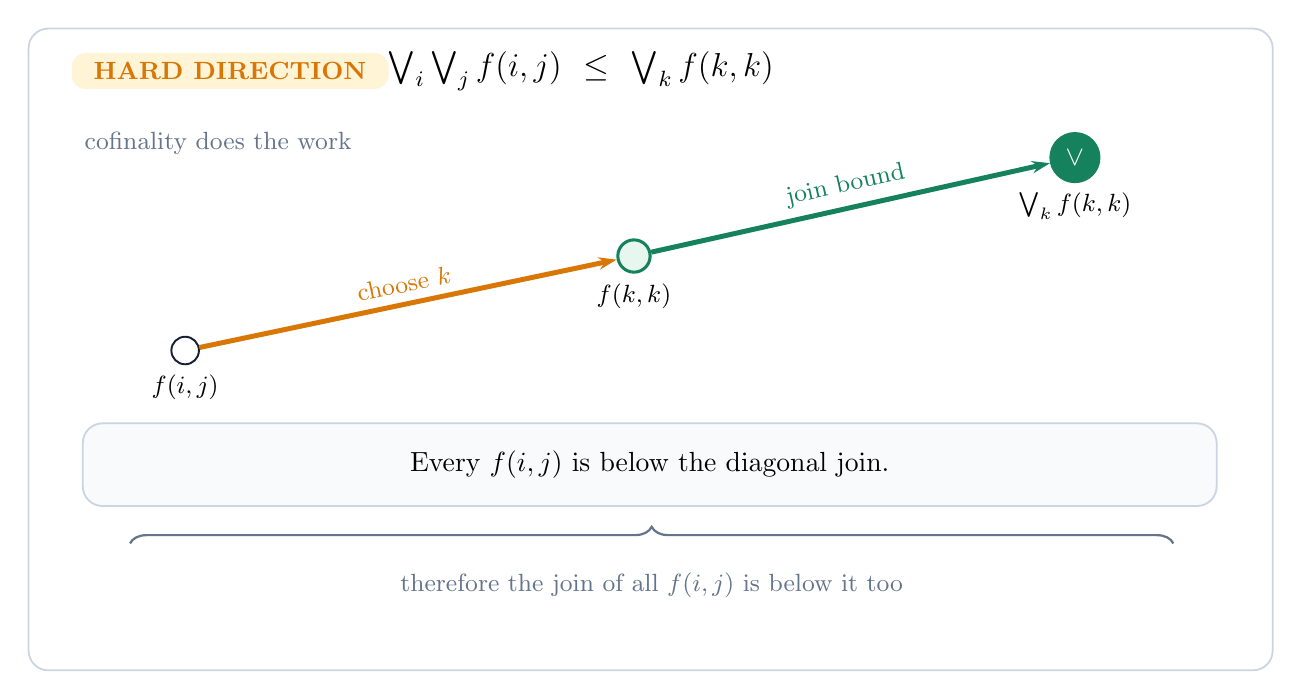
\begin{tikzpicture}[x=1cm,y=1cm]
  \node[card,minimum width=15.8cm,minimum height=8.15cm,anchor=north west] at (0,0) {};
  \node[pill,fill=amberpale,text=amber,anchor=west] at (.55,-.55) {HARD DIRECTION};
  \node[anchor=west,font=\bfseries\large] at (4.45,-.55)
    {$\Su_i\Su_j f(i,j)\ \le\ \Su_k f(k,k)$};
  \node[anchor=north west,font=\small,text=muted] at (.6,-1.2)
    {cofinality does the work};

  \node[point,label={[font=\small]below:$f(i,j)$}] (x) at (2.0,-4.1) {};
  \node[diagpoint,label={[font=\small]below:$f(k,k)$}] (d) at (7.7,-2.9) {};
  \node[circle,minimum size=5mm,draw=green,fill=green,text=white,
    label={[font=\small]below:$\Su_k f(k,k)$}] (s) at (13.3,-1.65) {$\vee$};
  \draw[->,amber,line width=1.8pt] (x)--node[above,sloped,font=\small] {choose $k$} (d);
  \draw[->,green,line width=1.8pt] (d)--node[above,sloped,font=\small] {join bound} (s);
  \node[card,fill=paper,minimum width=14.4cm,minimum height=1.05cm,align=center]
    at (7.9,-5.55) {Every $f(i,j)$ is below the diagonal join.};
  \draw[decorate,decoration={brace,amplitude=6pt},line width=.8pt,muted]
    (1.3,-6.55)--(14.55,-6.55) node[midway,below=7pt,font=\small,text=muted]
    {therefore the join of all $f(i,j)$ is below it too};
\end{tikzpicture}}
\end{minipage}\hfill
\begin{minipage}[t]{0.49\linewidth}
\resizebox{\linewidth}{!}{%
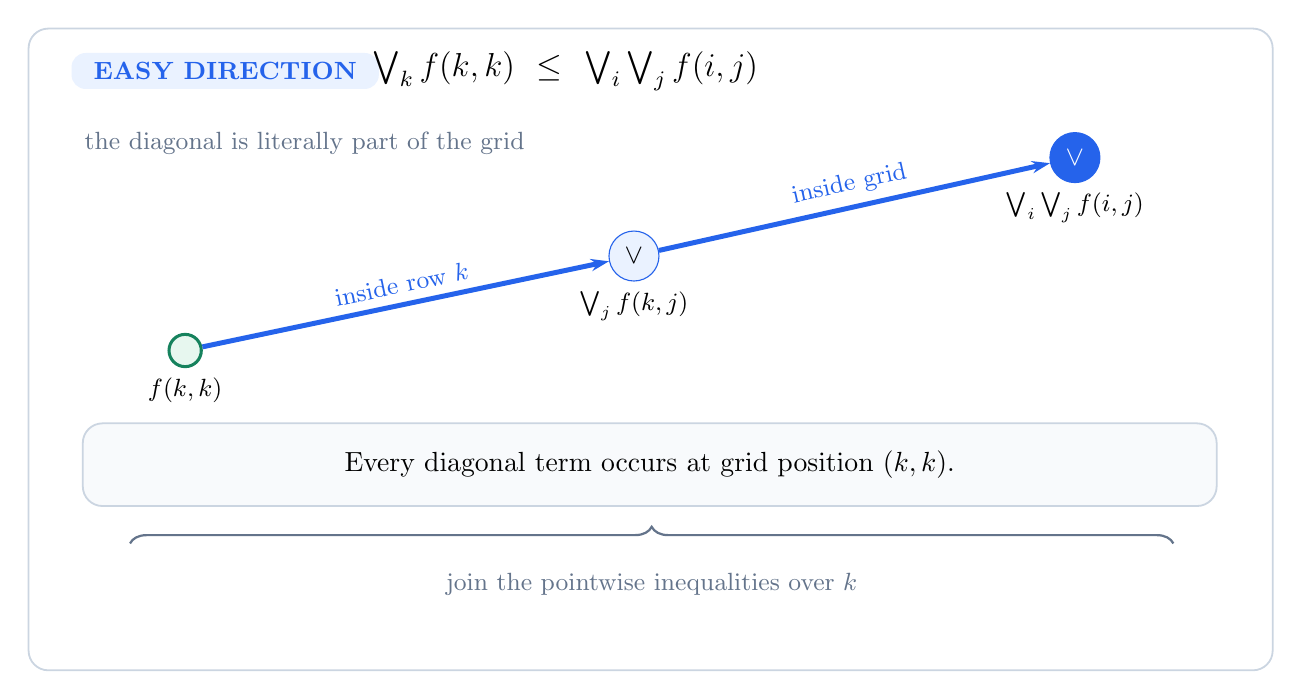
\begin{tikzpicture}[x=1cm,y=1cm]
  \node[card,minimum width=15.8cm,minimum height=8.15cm,anchor=north west] at (0,0) {};
  \node[pill,fill=bluepale,text=blue,anchor=west] at (.55,-.55) {EASY DIRECTION};
  \node[anchor=west,font=\bfseries\large] at (4.25,-.55)
    {$\Su_k f(k,k)\ \le\ \Su_i\Su_j f(i,j)$};
  \node[anchor=north west,font=\small,text=muted] at (.6,-1.2)
    {the diagonal is literally part of the grid};

  \node[diagpoint,label={[font=\small]below:$f(k,k)$}] (d) at (2.0,-4.1) {};
  \node[circle,minimum size=5mm,draw=blue,fill=bluepale,
    label={[font=\small]below:$\Su_j f(k,j)$}] (r) at (7.7,-2.9) {$\vee$};
  \node[circle,minimum size=5mm,draw=blue,fill=blue,text=white,
    label={[font=\small]below:$\Su_i\Su_j f(i,j)$}] (s) at (13.3,-1.65) {$\vee$};
  \draw[->,blue,line width=1.8pt] (d)--node[above,sloped,font=\small] {inside row $k$} (r);
  \draw[->,blue,line width=1.8pt] (r)--node[above,sloped,font=\small] {inside grid} (s);
  \node[card,fill=paper,minimum width=14.4cm,minimum height=1.05cm,align=center]
    at (7.9,-5.55) {Every diagonal term occurs at grid position $(k,k)$.};
  \draw[decorate,decoration={brace,amplitude=6pt},line width=.8pt,muted]
    (1.3,-6.55)--(14.55,-6.55) node[midway,below=7pt,font=\small,text=muted]
    {join the pointwise inequalities over $k$};
\end{tikzpicture}}
\end{minipage}

\vfill
\bigidea{Cofinality proves one side; inclusion of the diagonal proves the other.}

\newpage

% ------------------------------------------------------------------
% PAGE 3
\Title{Three duplicated proofs become one lattice move}{violet}

\resizebox{\linewidth}{!}{%
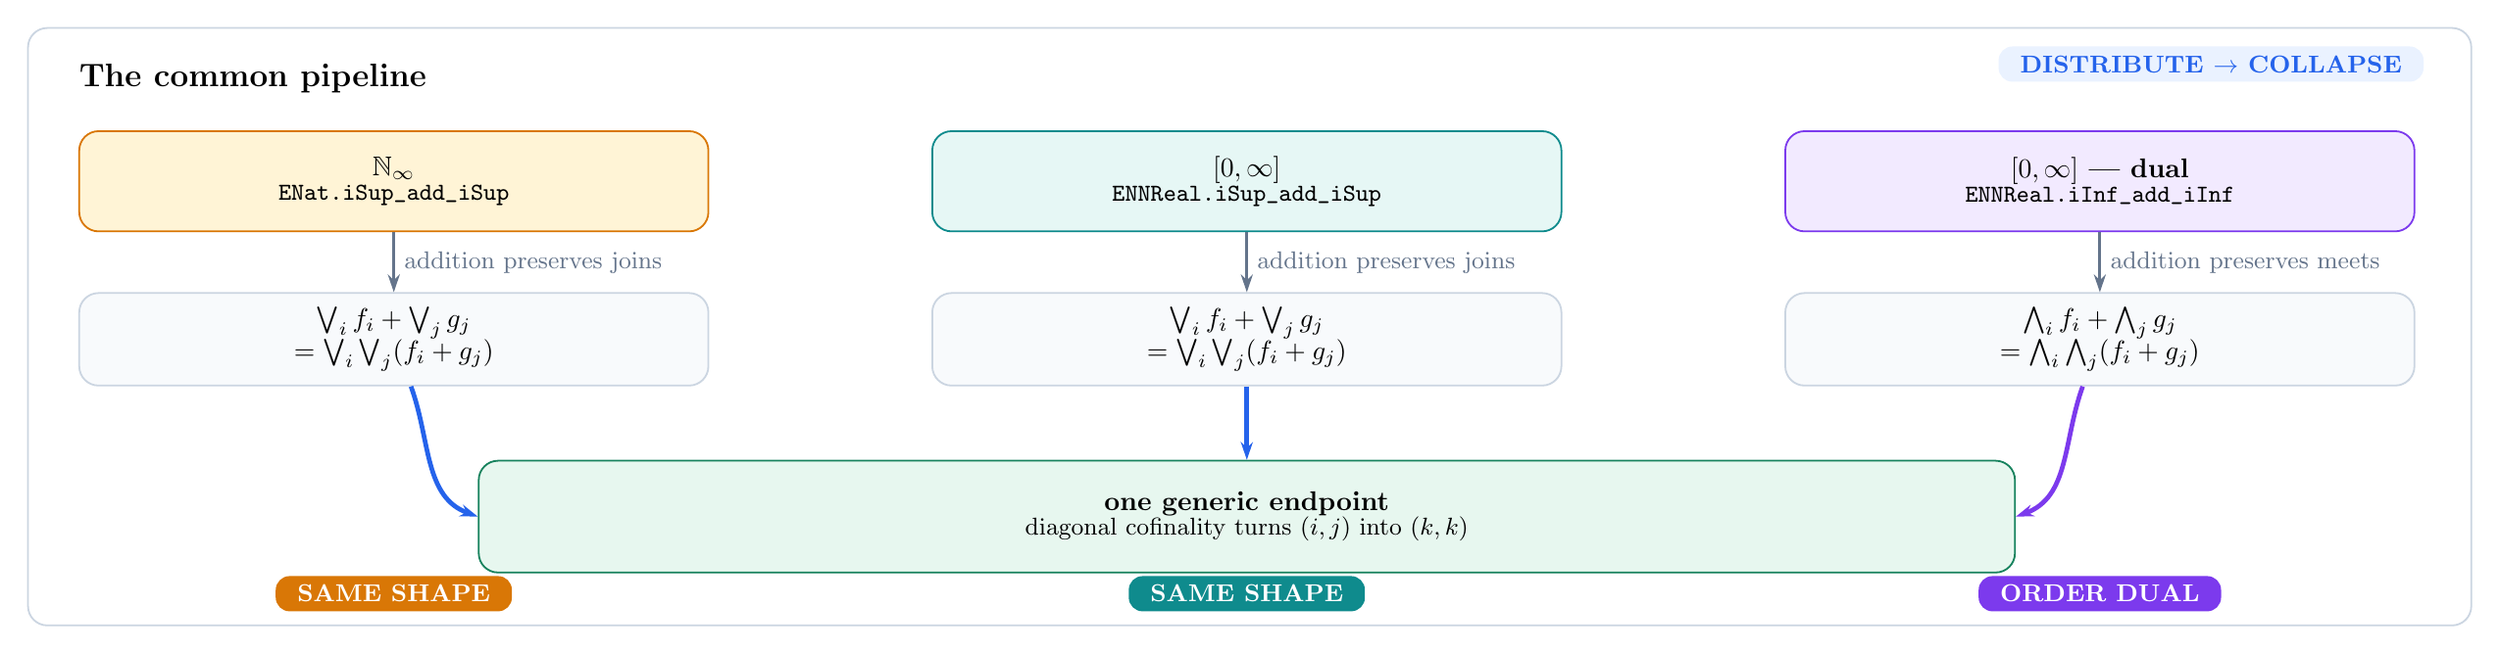
\begin{tikzpicture}[x=1cm,y=1cm]
  \node[card,minimum width=31.65cm,minimum height=7.75cm,anchor=north west] at (0,0) {};
  \node[anchor=north west,font=\bfseries\large] at (.55,-.35) {The common pipeline};
  \node[pill,fill=bluepale,text=blue,anchor=east] at (31.05,-.48) {DISTRIBUTE $\to$ COLLAPSE};

  \node[card,fill=amberpale,draw=amber,minimum width=8.15cm,minimum height=1.3cm,align=center]
    (enat) at (4.75,-2.0) {\bfseries $\mathbb N_\infty$\\[-1mm]\small \lean{ENat.iSup\char`_add\char`_iSup}};
  \node[card,fill=tealpale,draw=teal,minimum width=8.15cm,minimum height=1.3cm,align=center]
    (ennsup) at (15.8,-2.0) {\bfseries $[0,\infty]$\\[-1mm]\small \lean{ENNReal.iSup\char`_add\char`_iSup}};
  \node[card,fill=violetpale,draw=violet,minimum width=8.15cm,minimum height=1.3cm,align=center]
    (enninf) at (26.85,-2.0) {\bfseries $[0,\infty]$ --- dual\\[-1mm]\small \lean{ENNReal.iInf\char`_add\char`_iInf}};

  \node[card,fill=paper,minimum width=8.15cm,minimum height=1.2cm,align=center]
    (e1) at (4.75,-4.05) {$\Su_i f_i+\Su_j g_j$\\$=\Su_i\Su_j(f_i+g_j)$};
  \node[card,fill=paper,minimum width=8.15cm,minimum height=1.2cm,align=center]
    (e2) at (15.8,-4.05) {$\Su_i f_i+\Su_j g_j$\\$=\Su_i\Su_j(f_i+g_j)$};
  \node[card,fill=paper,minimum width=8.15cm,minimum height=1.2cm,align=center]
    (e3) at (26.85,-4.05) {$\In_i f_i+\In_j g_j$\\$=\In_i\In_j(f_i+g_j)$};
  \draw[flow] (enat)--node[right,font=\small] {addition preserves joins} (e1);
  \draw[flow] (ennsup)--node[right,font=\small] {addition preserves joins} (e2);
  \draw[flow] (enninf)--node[right,font=\small] {addition preserves meets} (e3);

  \node[card,fill=greenpale,draw=green,minimum width=19.9cm,minimum height=1.45cm,align=center]
    (core) at (15.8,-6.35) {\bfseries one generic endpoint\\[-1mm]
      \small diagonal cofinality turns $(i,j)$ into $(k,k)$};
  \draw[strongflow] (e1) to[out=-70,in=160] (core.west);
  \draw[strongflow] (e2)--(core);
  \draw[->,line width=1.7pt,color=violet] (e3) to[out=-110,in=20] (core.east);

  \node[pill,fill=amber,text=white] at (4.75,-7.35) {SAME SHAPE};
  \node[pill,fill=teal,text=white] at (15.8,-7.35) {SAME SHAPE};
  \node[pill,fill=violet,text=white] at (26.85,-7.35) {ORDER DUAL};
\end{tikzpicture}}

\vfill
\begin{minipage}[t]{0.465\linewidth}

\begin{tikzpicture}
  \node[card,minimum width=.99\linewidth,minimum height=1.48cm,anchor=north west] at (0,0) {};
  \node[pill,fill=rosepale,text=rose,anchor=west] at (.3,-.38) {BEFORE};
  \node[anchor=west,font=\small,align=left] at (2.65,-.38)
    {repeat nested-supremum bounds and witness chasing\\inside each numeric namespace};
\end{tikzpicture}
\end{minipage}\hfill
\begin{minipage}[t]{0.515\linewidth}

\begin{tikzpicture}
  \node[card,minimum width=.99\linewidth,minimum height=1.48cm,anchor=north west] at (0,0) {};
  \node[pill,fill=greenpale,text=green,anchor=west] at (.3,-.38) {AFTER};
  \node[anchor=west,font=\small,align=left,text=green] at (2.6,-.38)
    {{\ttfamily exact }\isupdiag{\ttfamily\ ... h}\\\color{muted}after the domain-specific distribution step};
\end{tikzpicture}
\end{minipage}

\newpage

% ------------------------------------------------------------------
% PAGE 4
\Title{The order-dual mirror gives the infimum theorem}{rose}

\begin{minipage}[t]{0.48\linewidth}
\resizebox{\linewidth}{!}{%
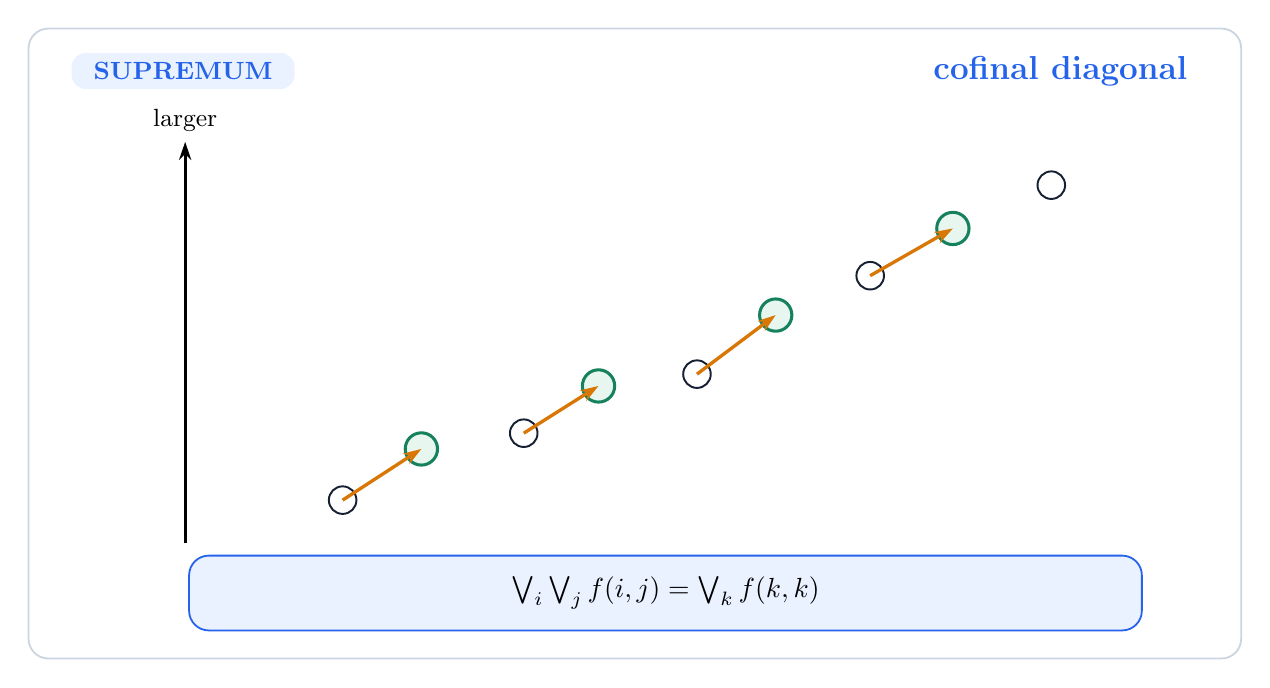
\begin{tikzpicture}[x=1cm,y=1cm]
  \node[card,minimum width=15.4cm,minimum height=8.0cm,anchor=north west] at (0,0) {};
  \node[pill,fill=bluepale,text=blue,anchor=west] at (.55,-.55) {SUPREMUM};
  \node[anchor=east,font=\bfseries\large,text=blue] at (14.85,-.55) {cofinal diagonal};
  \draw[->,line width=1pt] (2.0,-6.55)--(2.0,-1.45) node[above,font=\small] {larger};
  \foreach \x/\y in {4.0/-6.0,6.3/-5.15,8.5/-4.4,10.7/-3.15,13.0/-2.0}
    {\node[point] at (\x,\y) {};}
  \foreach \x/\y in {5.0/-5.35,7.25/-4.55,9.5/-3.65,11.75/-2.55}
    {\node[diagpoint] at (\x,\y) {};}
  \draw[->,amber,line width=1.2pt] (4.0,-6.0)--(5.0,-5.35);
  \draw[->,amber,line width=1.2pt] (6.3,-5.15)--(7.25,-4.55);
  \draw[->,amber,line width=1.2pt] (8.5,-4.4)--(9.5,-3.65);
  \draw[->,amber,line width=1.2pt] (10.7,-3.15)--(11.75,-2.55);
  \node[card,fill=bluepale,draw=blue,minimum width=12.1cm,minimum height=.95cm]
    at (8.1,-7.18) {$\Su_i\Su_j f(i,j)=\Su_k f(k,k)$};
\end{tikzpicture}}
\end{minipage}\hfill
\begin{minipage}[t]{0.48\linewidth}
\resizebox{\linewidth}{!}{%
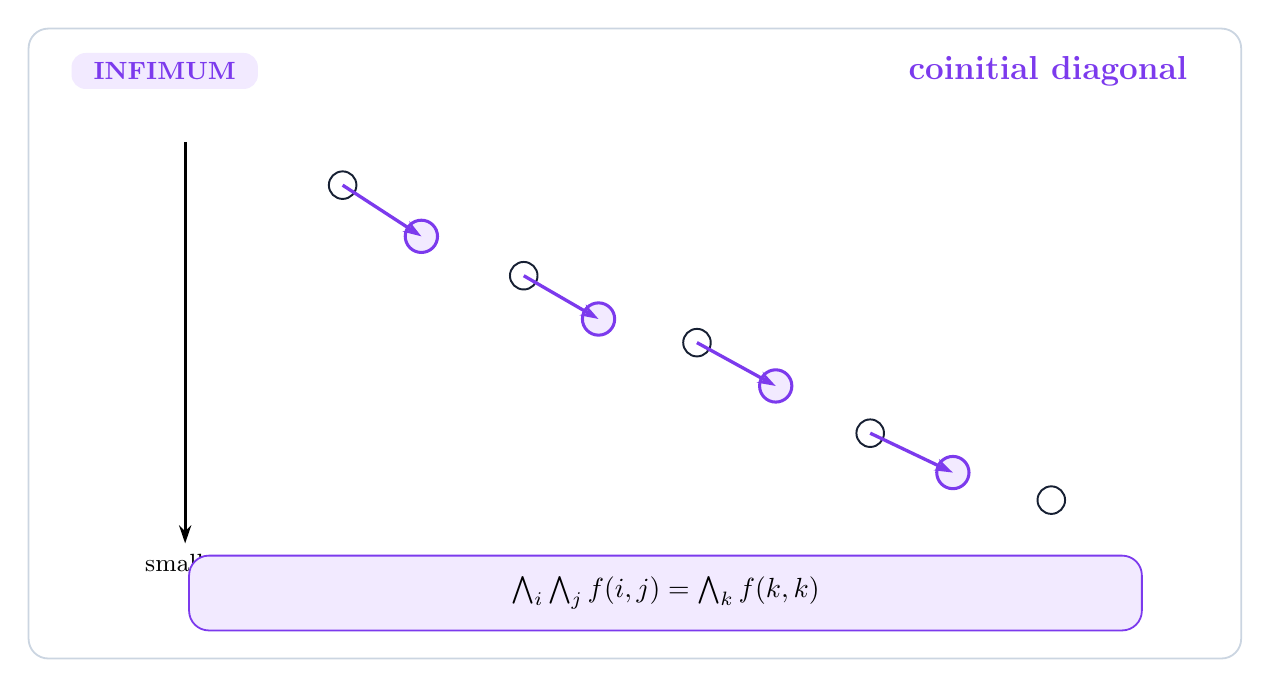
\begin{tikzpicture}[x=1cm,y=1cm]
  \node[card,minimum width=15.4cm,minimum height=8.0cm,anchor=north west] at (0,0) {};
  \node[pill,fill=violetpale,text=violet,anchor=west] at (.55,-.55) {INFIMUM};
  \node[anchor=east,font=\bfseries\large,text=violet] at (14.85,-.55) {coinitial diagonal};
  \draw[->,line width=1pt] (2.0,-1.45)--(2.0,-6.55) node[below,font=\small] {smaller};
  \foreach \x/\y in {4.0/-2.0,6.3/-3.15,8.5/-4.0,10.7/-5.15,13.0/-6.0}
    {\node[point] at (\x,\y) {};}
  \foreach \x/\y in {5.0/-2.65,7.25/-3.7,9.5/-4.55,11.75/-5.65}
    {\node[diagpoint,draw=violet,fill=violetpale] at (\x,\y) {};}
  \draw[->,violet,line width=1.2pt] (4.0,-2.0)--(5.0,-2.65);
  \draw[->,violet,line width=1.2pt] (6.3,-3.15)--(7.25,-3.7);
  \draw[->,violet,line width=1.2pt] (8.5,-4.0)--(9.5,-4.55);
  \draw[->,violet,line width=1.2pt] (10.7,-5.15)--(11.75,-5.65);
  \node[card,fill=violetpale,draw=violet,minimum width=12.1cm,minimum height=.95cm]
    at (8.1,-7.18) {$\In_i\In_j f(i,j)=\In_k f(k,k)$};
\end{tikzpicture}}
\end{minipage}

\vfill
\begin{center}

\begin{tikzpicture}
  \node[pill,fill=blue,text=white] (sup) {\isupdiag};
  \node[pill,fill=ink,text=white,right=2.1cm of sup] (dual) {REVERSE $\le$};
  \node[pill,fill=violet,text=white,right=2.1cm of dual] (inf) {\iinfdiag};
  \draw[<->,line width=1.2pt,color=muted] (sup)--node[above,font=\small] {order duality} (dual);
  \draw[<->,line width=1.2pt,color=muted] (dual)--node[above,font=\small] {automatic twin} (inf);
\end{tikzpicture}
\end{center}

\newpage

% ------------------------------------------------------------------
% PAGE 5
\Title{When does the diagonal condition appear naturally?}{amber}

\begin{minipage}[t]{0.58\linewidth}
\resizebox{\linewidth}{!}{%
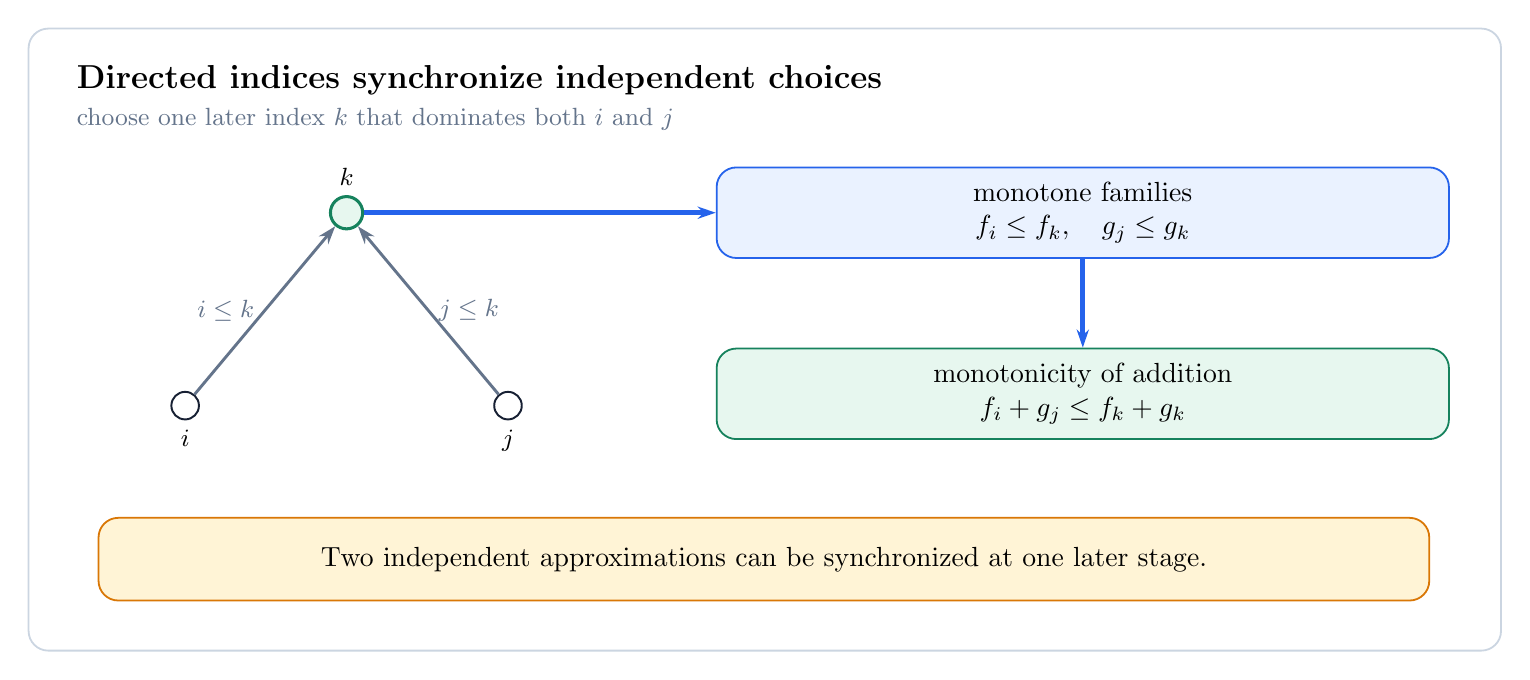
\begin{tikzpicture}[x=1cm,y=1cm]
  \node[card,minimum width=18.7cm,minimum height=7.9cm,anchor=north west] at (0,0) {};
  \node[anchor=north west,font=\bfseries\large] at (.5,-.35) {Directed indices synchronize independent choices};
  \node[anchor=north west,font=\small,text=muted] at (.5,-.9)
    {choose one later index $k$ that dominates both $i$ and $j$};

  \node[point,label={[font=\small]below:$i$}] (i) at (2.0,-4.8) {};
  \node[point,label={[font=\small]below:$j$}] (j) at (6.1,-4.8) {};
  \node[diagpoint,label={[font=\small]above:$k$}] (k) at (4.05,-2.35) {};
  \draw[flow] (i)--node[left,font=\small] {$i\le k$} (k);
  \draw[flow] (j)--node[right,font=\small] {$j\le k$} (k);

  \node[card,fill=bluepale,draw=blue,minimum width=9.3cm,minimum height=1.15cm,align=center]
    (mono) at (13.4,-2.35) {monotone families\\$f_i\le f_k,\quad g_j\le g_k$};
  \node[card,fill=greenpale,draw=green,minimum width=9.3cm,minimum height=1.15cm,align=center]
    (add) at (13.4,-4.65) {monotonicity of addition\\$f_i+g_j\le f_k+g_k$};
  \draw[strongflow] (k)--(mono);
  \draw[strongflow] (mono)--(add);

  \node[card,fill=amberpale,draw=amber,minimum width=16.9cm,minimum height=1.05cm,align=center]
    at (9.35,-6.75) {Two independent approximations can be synchronized at one later stage.};
\end{tikzpicture}}
\end{minipage}\hfill
\begin{minipage}[t]{0.405\linewidth}
\resizebox{\linewidth}{!}{%
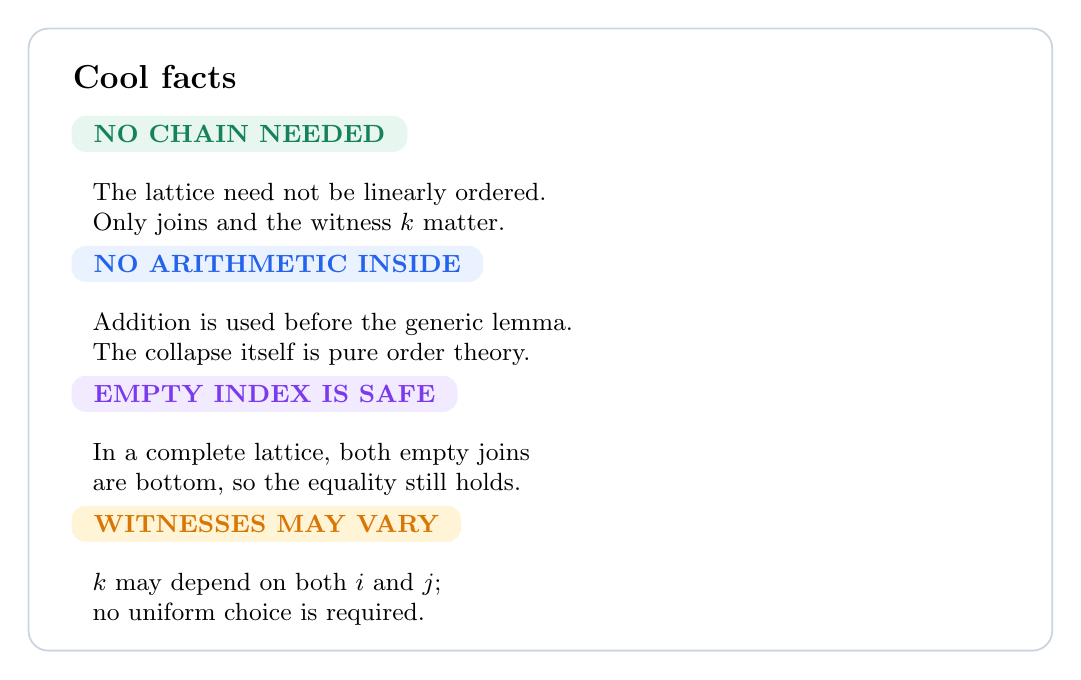
\begin{tikzpicture}[x=1cm,y=1cm]
  \node[card,minimum width=13.0cm,minimum height=7.9cm,anchor=north west] at (0,0) {};
  \node[anchor=north west,font=\bfseries\large] at (.45,-.35) {Cool facts};

  \node[pill,fill=greenpale,text=green,anchor=west] at (.55,-1.35) {NO CHAIN NEEDED};
  \node[anchor=north west,font=\small,align=left] at (.7,-1.85)
    {The lattice need not be linearly ordered.\\Only joins and the witness $k$ matter.};

  \node[pill,fill=bluepale,text=blue,anchor=west] at (.55,-3.0) {NO ARITHMETIC INSIDE};
  \node[anchor=north west,font=\small,align=left] at (.7,-3.5)
    {Addition is used before the generic lemma.\\The collapse itself is pure order theory.};

  \node[pill,fill=violetpale,text=violet,anchor=west] at (.55,-4.65) {EMPTY INDEX IS SAFE};
  \node[anchor=north west,font=\small,align=left] at (.7,-5.15)
    {In a complete lattice, both empty joins\\are bottom, so the equality still holds.};

  \node[pill,fill=amberpale,text=amber,anchor=west] at (.55,-6.3) {WITNESSES MAY VARY};
  \node[anchor=north west,font=\small,align=left] at (.7,-6.8)
    {$k$ may depend on both $i$ and $j$;\\no uniform choice is required.};
\end{tikzpicture}}
\end{minipage}

\vfill
\bigidea{The lemma packages the synchronization step, not the domain-specific algebra.}

\newpage

% ------------------------------------------------------------------
% PAGE 6
\Title{Why this is an upstream-sized contribution}{green}

\begin{minipage}[t]{0.57\linewidth}
\resizebox{\linewidth}{!}{%
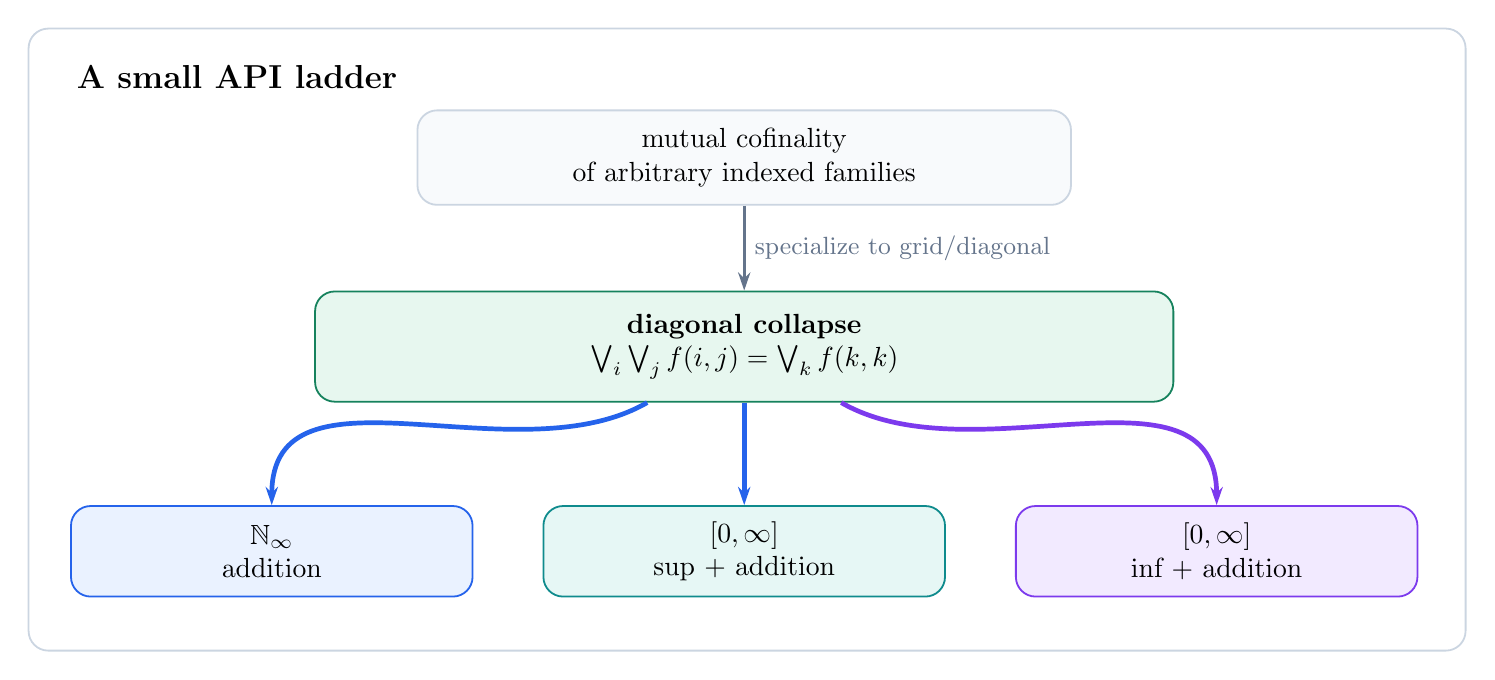
\begin{tikzpicture}[x=1cm,y=1cm]
  \node[card,minimum width=18.25cm,minimum height=7.9cm,anchor=north west] at (0,0) {};
  \node[anchor=north west,font=\bfseries\large] at (.5,-.35) {A small API ladder};

  \node[card,fill=paper,minimum width=8.3cm,minimum height=1.2cm,align=center]
    (cof) at (9.1,-1.65) {mutual cofinality\\of arbitrary indexed families};
  \node[card,fill=greenpale,draw=green,minimum width=10.9cm,minimum height=1.4cm,align=center]
    (diag) at (9.1,-4.05) {\bfseries diagonal collapse\\$\Su_i\Su_j f(i,j)=\Su_k f(k,k)$};
  \node[card,fill=bluepale,draw=blue,minimum width=5.1cm,minimum height=1.15cm,align=center]
    (enat) at (3.1,-6.65) {$\mathbb N_\infty$\\addition};
  \node[card,fill=tealpale,draw=teal,minimum width=5.1cm,minimum height=1.15cm,align=center]
    (ennsup) at (9.1,-6.65) {$[0,\infty]$\\sup + addition};
  \node[card,fill=violetpale,draw=violet,minimum width=5.1cm,minimum height=1.15cm,align=center]
    (enninf) at (15.1,-6.65) {$[0,\infty]$\\inf + addition};
  \draw[flow] (cof)--node[right,font=\small] {specialize to grid/diagonal} (diag);
  \draw[strongflow] (diag) to[out=-150,in=90] (enat);
  \draw[strongflow] (diag)--(ennsup);
  \draw[->,line width=1.7pt,color=violet] (diag) to[out=-30,in=90] (enninf);
\end{tikzpicture}}
\end{minipage}\hfill
\begin{minipage}[t]{0.415\linewidth}
\resizebox{\linewidth}{!}{%
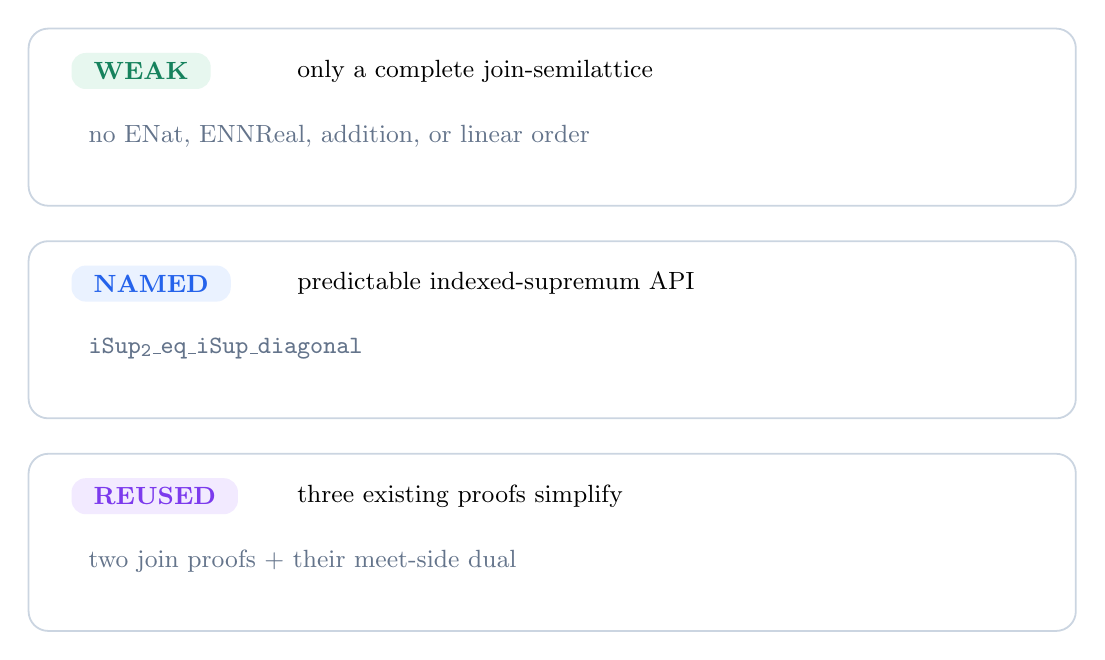
\begin{tikzpicture}[x=1cm,y=1cm]
  \node[card,minimum width=13.3cm,minimum height=2.25cm,anchor=north west] at (0,0) {};
  \node[pill,fill=greenpale,text=green,anchor=west] at (.55,-.55) {WEAK};
  \node[anchor=west,font=\small] at (3.3,-.55) {only a complete join-semilattice};
  \node[anchor=west,font=\small,text=muted] at (.65,-1.38)
    {no ENat, ENNReal, addition, or linear order};

  \node[card,minimum width=13.3cm,minimum height=2.25cm,anchor=north west] at (0,-2.7) {};
  \node[pill,fill=bluepale,text=blue,anchor=west] at (.55,-3.25) {NAMED};
  \node[anchor=west,font=\small] at (3.3,-3.25) {predictable indexed-supremum API};
  \node[anchor=west,font=\small,text=muted] at (.65,-4.08)
    {\isupdiag};

  \node[card,minimum width=13.3cm,minimum height=2.25cm,anchor=north west] at (0,-5.4) {};
  \node[pill,fill=violetpale,text=violet,anchor=west] at (.55,-5.95) {REUSED};
  \node[anchor=west,font=\small] at (3.3,-5.95) {three existing proofs simplify};
  \node[anchor=west,font=\small,text=muted] at (.65,-6.78)
    {two join proofs + their meet-side dual};
\end{tikzpicture}}
\end{minipage}

\vfill
\begin{center}

\begin{tikzpicture}[node distance=1.15cm]
  \node[pill,fill=ink,text=white] (spot) {SPOT THE GRID};
  \node[pill,fill=amberpale,text=amber,right=of spot] (erase) {ERASE ARITHMETIC};
  \node[pill,fill=greenpale,text=green,right=of erase] (name) {NAME DIAGONAL COLLAPSE};
  \node[pill,fill=bluepale,text=blue,right=of name] (reuse) {REFACTOR 3 PROOFS};
  \draw[flow] (spot)--(erase); \draw[flow] (erase)--(name); \draw[flow] (name)--(reuse);
\end{tikzpicture}
\end{center}

\end{document}
